\documentclass[a4paper,12pt]{article}
\usepackage{amsmath}
\usepackage{graphicx}
\usepackage{bm}

\graphicspath{ {.} }
\begin{document}

\begin{center}
\Huge The process of minimizing the error function within Machine Learning \\
\small Mathematics HL Internal Assessment
\end{center}

\section{Rationale}
This mathematical exploration focuses on the process of minimizing the error of a neural network, a big part of the machine learning field. Machine learning and artificial intelligence has always stood out to me given its apparent complexity and increasing usage. I've always been fascinated by computer's and mathemtical model's ability to learn from past experience, something that has always been regarded as an ultimately human trait. I want to investigate how calculus, and in particular the chain rule, is being applied to these models and what it is that these different methods of minimizing the error function is eventually achieving. 

\section{Notation}
The notation \(m\) means the number of training sets. \\
The notation \(n\) means the number of weights in the network.  \\
The notation $x^{(i)}$ means input, of the $i$-th training set.  \\
The notation $y^{(i)}$ means output, of the $i$-th training set.  \\
The notation $y$ means output, while $\boldsymbol{y}$ means the row vector of all outputs, dimension m $\times$ 1. \\
The notation $\boldsymbol{X}$ means the matrix collection of all inputs and features, of dimension $m \times n$.\\
The notation $\boldsymbol{X}^t_s$ means the $t$-th row, and $s$-th column of the matrix $\boldsymbol{X}$. \\
The notation \boldmath{$\Theta$}\unboldmath \ means the matrix collection of weights of the model. \\
The notation $\theta_{jk}^l$ means the weight connecting neuron $j$ to $k$, in layer $l$. \\
The notation $b_j^l$ means the bias connected to neuron $j$, in layer $l$. Also noted as $\theta^l_0$ with reference to no previous connection.\\
The notation $z_j^l$ means the value gained from the hypothesis function. \\
The notation $\sigma$ means the activation function. \\
The notation $a^l_j$ means the activation of neuron $j$, in layer $l$. 

\section{Introduction on neural networks}
An artificial neural network is defined as 'a computer system modelled on the human brain and nervous system' \cite{nndef}. In a sentence, a neural network is a collection of input, hidden and output layers whose values are determined through learning. The process is that given some input $x$ the network will give an output \(y\), which follows a mathematical model that learns from previous experiences. The neural network setup has three layers. The first layer is the input layer, a matrix \textbf{\emph{X}} of \(n\) inputs \(x_0,x_1,...x_n\). The full input matrix then takes on multiple training sets, resulting in the dimension of $m \times n$. The input layer is simply the values that are put into the network, or the data. The second layer is the hidden layer where there is a collection of weights(\(\boldsymbol{\Theta}\)) and biases, which are manipulated, in terms of adjusting parameters, by the machine learning algorithm from training sets to introduce the most accurate model. The hidden layer is anything that is not a part of the input and output layers and can include any number of them. The last layer is the output layer which gives out the output, \(y\). The weights in the hidden layer take on a certain activation value based on a hypothesis function that gets run through an activation function. The collection of values from the previous layer then gets transitioned to the next layer, into each weight and new values are computed. The weights end up making a decision on a regression or classification problem. A regression problem deals with continuous problems, for example deciding the price of a certain size of a new house given data about housing prices and sizes in the region. A classification problem deals with classifying the data. For example, deciding if an image is an apple or an orange. At the output layer, these decisions would be given \cite{patternml}.

\section{Modelling}
To go with the example of housing prices, a simple example of a regression problem would be finding a good hypothesis function \(h_{\boldsymbol{\Theta}}(x)\) so that it predicts the price the house would sell at, given the input $\boldsymbol{X}$. If we take in a single-variable input on the size of the house, the model is linear on the form  \(h_\theta(x) = \theta_0 + \theta_1x\) where the parameters \(\theta_0\) and \(\theta_1\) are the ideal values to minimize the error, which is noted \(J(\theta\)). The goal is that given our training set to learn the weights for our hypothesis function. However, given multiple input variables, the model is \(h_{\boldsymbol{\theta}(x)} = \theta_0x_0 + \theta_1x_1 + ... + \theta_nx_n\) \cite{patternml}. For mathematical convenience, a value $x_0$ is introduced to be set to 1, to simplify the model to:
\[h_{\boldsymbol{\Theta}}(x) = \sum_{i = 0}^m \theta_ix_i\]

\section{The error function}
\[J(\boldsymbol{\Theta}) = \frac{1}{2m} \sum_{i=1}^m (h_\theta(x^{(i)}) - y^{(i)})^2\]
The key to creating accurate models is the error function from the training data. There are multiple ways to represent the error in prediction, but objectively the most popularly used one is the square-error function, as the squared error puts more emphasis on the weights and biases that influence the model the most, as the value is squared \cite{patternml}. The function takes the predicted value by the model and subtracts the predetermined value known by the training set, squaring both. The half is for mathematical convenience when deriving. However, the error function is computed for the of $m$ number of training sets. 
The square-error function is easy to minimize given its convexity \cite{convex}. The function is convex, which means that there is only a single minimum which simplifies the process of finding the minimum. Through minimizing the error function, the ideal weights can be found, and the model can be applied to be the best fit, as the lowest value of the error function is the lowest discrepancy between the prediction and the result..

\section{The activation function}
At each neuron in the neural network, the previous layer of neurons get multiplied by the weight connecting them to the neurons in the next layer. Mathematically, that is given by our hypothesis function of $h_{\boldsymbol{\Theta}}(x)$. The value then gets run through an activation function. The activation function, $S(x)$, makes the expression non-linear and binds it to a range. A well-used function is the sigmoid, which binds the activation output into a range between 0 and 1 \cite{patternml}. The sigmoid is given by, and takes on the following graph:
\[S(x) = \frac{1}{1+e^{-x}}\]
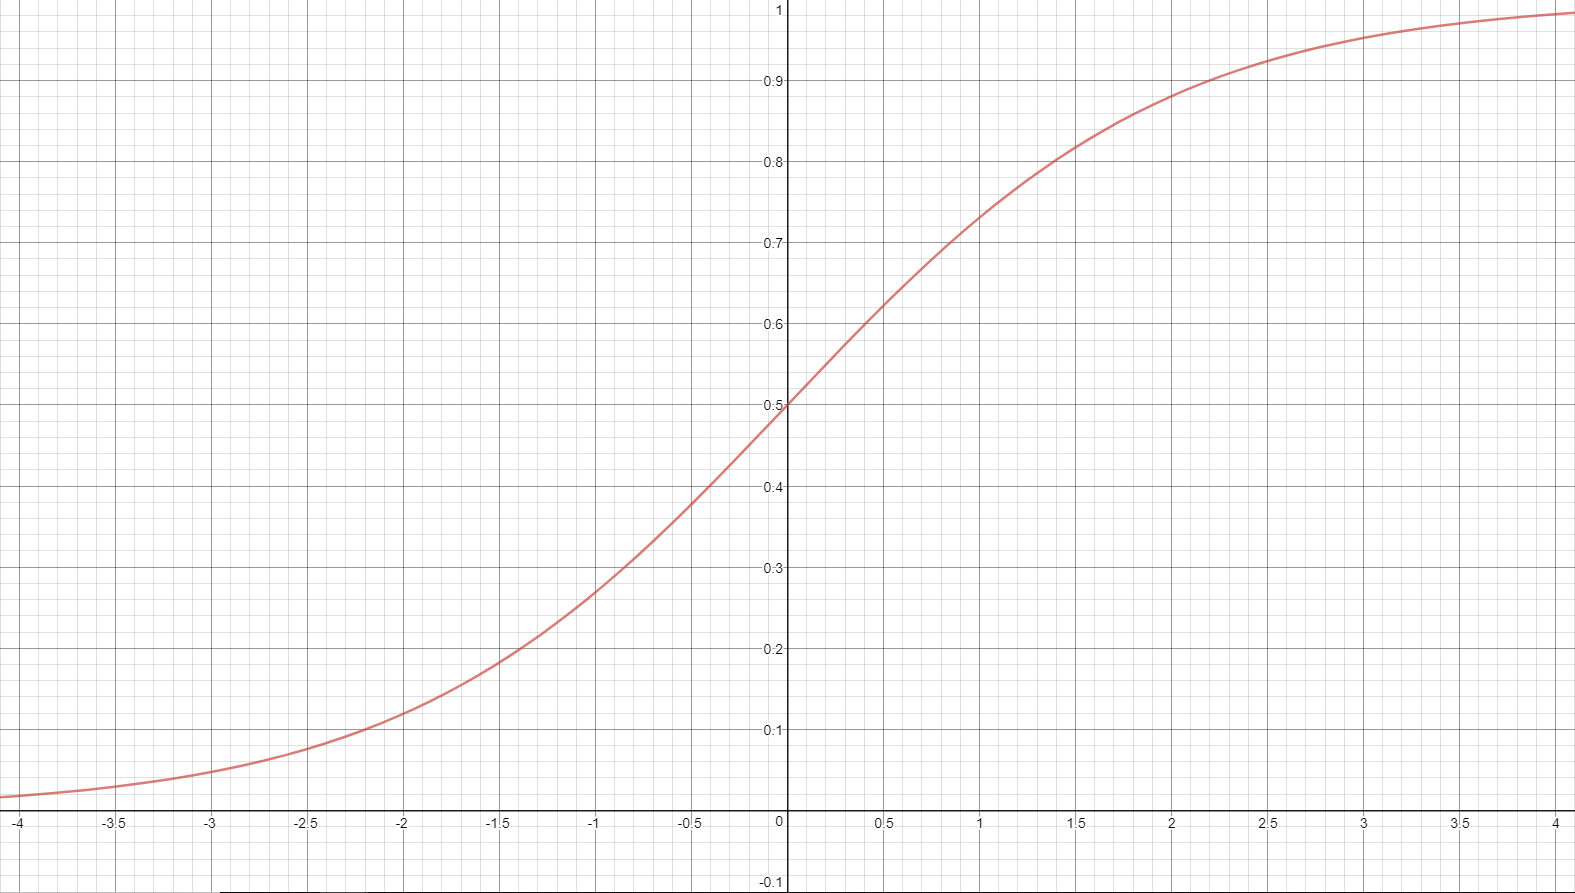
\includegraphics[scale=0.25]{sigmoid}
\textbf{Figure 1.} The graphical representation of the sigmoid/activation function.\\

In the process of backpropagation, which will be explained in further depth later, it is important the activation function is differentiable. The sigmoid function can be derived \cite{backpropagation}, and will come in handy later:
\[\frac{dS}{dx} = \frac{d}{dx}(1+e^{-x})^{-1}\]
\[\frac{dS}{dx} = -1(1+e^{-x})^{-1-1} \times -1 \times e^{-x}\]
\[\frac{dS}{dx} = e^{-x}(1+e^{-x})^{-2}\]
\[\frac{dS}{dx} = \frac{e^{-x}}{(1+e^{-x})^2}\]
\[\frac{dS}{dx} = \frac{1 + e^{-x} - 1}{(1+e^{-x})^2}\]
\[\frac{dS}{dx} = \frac{1}{1+e^{-x}}\bigg[\frac{1+e^{-x}}{1+e^{-x}} - \frac{1}{1+e^{-x}}\bigg] \]
\[\frac{dS}{dx} = \sigma' = S(1-S)\]

\section{Gradient Descent}
The goal of the gradient descent algorithm is to minimize the error function by using the tangent line at an initial point, and moving into the direction of the negative gradient, toward a local minimum until the gradient is zero at a local minimum. If the function is convex and upcave, that point is going to be the global minimum, but if the function is not convex, the reached minimum will depend on the starting point and not necessarily be a global minimum. The algorithm is defined as \cite{deeplearning} \[\theta_j = \theta_j - \alpha \frac{\partial}{\partial\theta_j} J(\boldsymbol{\Theta})\] The \(\alpha\) marks the learning rate, which gives the difference between the points. A higher learning rate means a bigger jump, which if high enough can result in overshooting the local minimum and failing to converge. A smaller learning rate means the opposite but will be computationally more difficult. The learning rate gets multiplied by the partial derivative of to error function, with respect to the current parameter. 

The partial derivative of a multi-input function, is its derivative with respect to one of its inputs, where the other inputs are held constant. 

The algorithm gets repeated for every parameter at once and moves accordingly. However, to get a complete algorithm, the error function must be partially derived. 
\\
\\
\textbf{Theorem 1 \cite{sumrule}:} The sum rule. The derived sum of all terms is the same as the sum of all terms derived, given a finite sum.
\[(f(x) + g(x))^{'} = f(x)^{'} + g(x)^{'} \]
\textbf{Proof:} As by the first priniciple, $f(x)$ and $g(x)$ can be noted as:
\[((f(x)+h(x))^{'} = \lim_{h\to\infty} \frac{f(x+h) - f(x) + g(x+h) - g(x)}{h}\] 
\[= \lim_{h\to\infty} \frac{f(x+h) - f(x)}{h} + \lim_{h\to\infty} \frac{g(x+h) - g(x)}{h}\]
\[= f^{'}(x) + g^{'}(x)\]
\\
The theorem allows us to successfully differentiate the error function, which includes a sum:
\[J(\boldsymbol{\Theta}) = \frac{1}{2m} \sum_{i=1}^m (h_{\boldsymbol{\Theta}}(x^{(i)}) - y^{(i)})^2\]
Here the sum rule gets applied, as the sum of derivatives is equal to the derivative of the sums, the sum can be ignored during the process:
\[\frac{\partial}{\partial\theta_j} [J(\boldsymbol{\Theta})] = \frac{\partial}{\partial\theta_j} \Big[ \frac{1}{2m} \sum_{i=1}^m (h_{\boldsymbol{\Theta}}(x^{(i)}) - y^{(i)})^2\Big]\]
\[\frac{\partial}{\partial\theta_j} [J(\boldsymbol{\Theta})] = \frac{1}{2m} \sum_{i=1}^m \frac{\partial}{\partial\theta_j} [h_{\boldsymbol{\Theta}}(x^{(i)}) - y^{(i)})^2]\]
\[\frac{\partial}{\partial\theta_j} [J(\boldsymbol{\Theta})] = \frac{1}{2m} \sum_{i=1}^m 2(h_{\boldsymbol{\Theta}}(x^{(i)}) - y^{(i)}) \frac{\partial}{\partial\theta_j}[h_{\boldsymbol{\Theta}}(x^{(i)}) - y^{(i)}]\]
\[\frac{\partial}{\partial\theta_j} [J(\boldsymbol{\Theta})] = \frac{1}{m} \sum_{i=1}^m (h_{\boldsymbol{\Theta}}(x^{(i)}) - y^{(i)})\frac{\partial}{\partial\theta_j} [\theta_0x_0^{(i)}+\theta_1x_1^{(i)}+...+\theta_nx_n^{(i)}-y^{(i)}]\]
For the final step, we partially derive on the right hand-side, with respect to $\theta_j$. The arbitrary value $j$ derives for the arbitrary expression $\theta_jx_j^{(i)}$, while keeping the other inputs as constants. The resulting partial derivative, therefore, is $x_j^{(i)}$.
\[\frac{\partial}{\partial\theta_j} [J(\boldsymbol{\Theta})] = \frac{1}{m} \sum_{i=1}^m (h_{\boldsymbol{\Theta}}(x^{(i)}) - y^{(i)})x_j^{(i)}\]
The final algorithm is therefore \cite{deeplearning}:
\[\theta_j = \theta_j - \alpha \frac{1}{m} \sum_{i=1}^m (h_{\boldsymbol{\Theta}}(x^{(i)} - y^{(i)})x_j^{(i)} \ \text{for} \ j = 0,1,...,n\]
\\
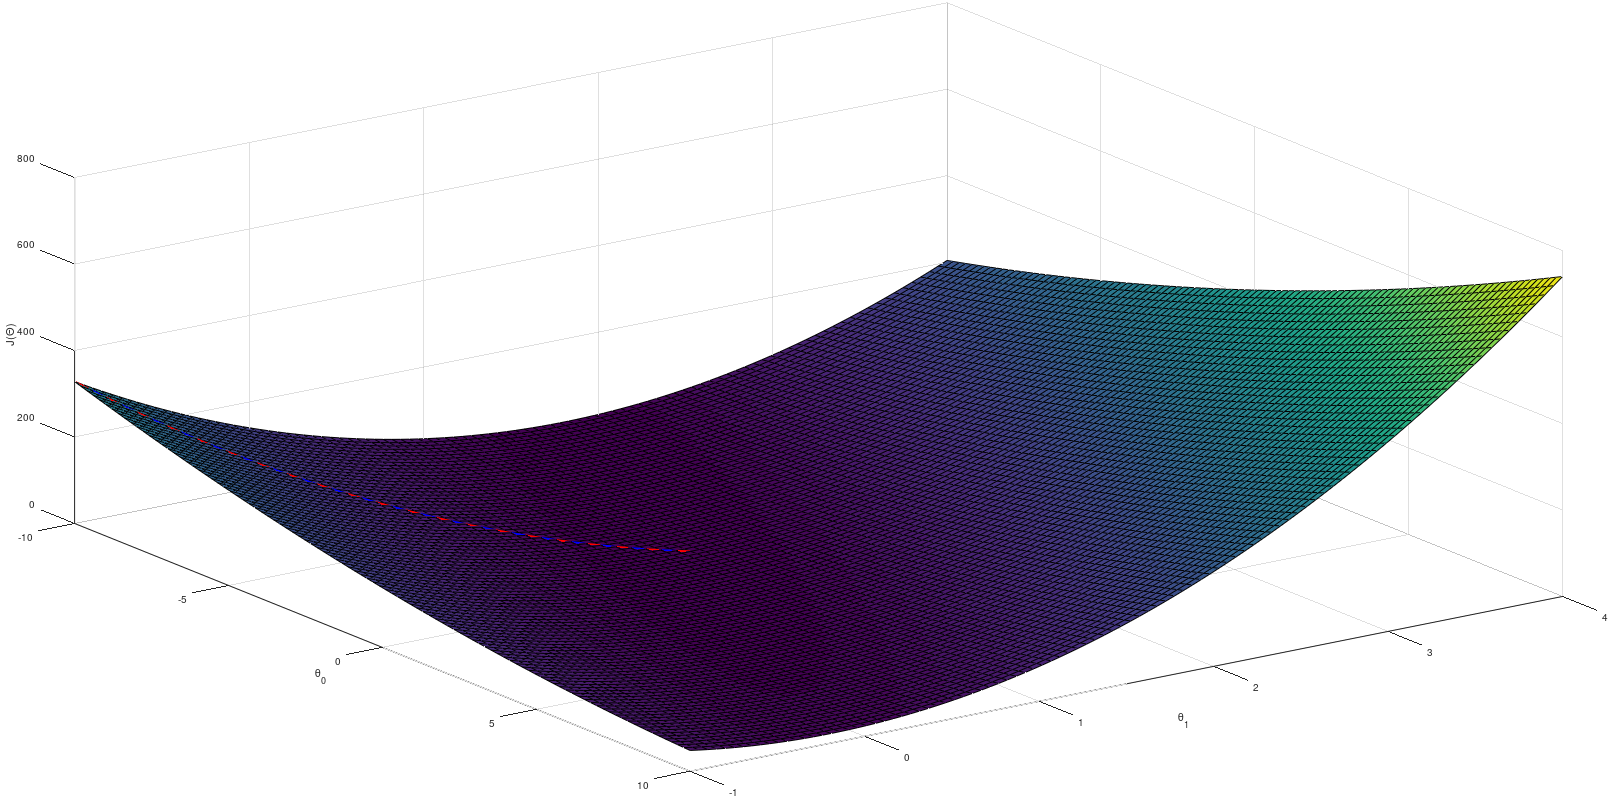
\includegraphics[scale=0.38]{gradientdescent}
\textbf{Figure 2.} The application of the algorithm can be visualized on this diagram. The diagram shows the $x$-axis and $y$-axis as the weights $\theta_0$ and $\theta_1$, while the $z$ axis is the error cost function, $J(\boldsymbol{\Theta})$. The scale of the $x$-axis is $5$, the $y$-axis is $1$ and the $z$-axis is $200$. The path the algorithm takes to the minimum is visualized, with each step being represented by either blue or red.
\\
\section{Normal equations}
A more analytical way to compute the global minimum of the convex error function is by using normal equations. The normal equation gives the parameters for a minimized error function and is defined as \cite{normal}
\[\boldsymbol{\Theta} = (\boldsymbol{X}^T\boldsymbol{X})^{-1}\boldsymbol{X}^T\boldsymbol{y}\]
The theta refers to the matrix containing the minimized \(\theta_j\) values, or weights. The matrix \boldsymbol{$X$} is the input matrix $m \times n$, while the matrix \boldsymbol{$y$} \ is the known result from the training set, dimension $m \times 1$. 
\\

The notation $\boldsymbol{X}^T$ means to take the transpose of the matrix $\boldsymbol{X}$. The transpose operation means to interchange the rows and the columns of a matrix. The rows become columns, and columns become rows. 
\\

By taking the squared error function and transforming it into a vectorized format we have:
\[\begin{bmatrix} h_{\boldsymbol{\Theta}} (\boldsymbol{X}^0) - y^0 \\ h_{\boldsymbol{\Theta}} (\boldsymbol{X}^1) - y^1 \\ h_{\boldsymbol{\Theta}} (\boldsymbol{X}^2) - y^2 \\ . \\ . \\ . \\  \\ h_{\boldsymbol{\Theta}} (\boldsymbol{X}^m) - y^m\end{bmatrix}\]
where $h_{\boldsymbol{\Theta}} (\boldsymbol{X}^0)$ is the hypothesis function for an individual training set, or for a two feature example, $h_{\boldsymbol{\Theta}} (x_0, x_1, x_2) = \theta_0x_0 + \theta_1x_1 + \theta_2x_2 = 10\times 1 + 25 \times 3 + 42 \times 2$. As per the error function, the value for $h_{\boldsymbol{\Theta}} (\boldsymbol{X}^m)$ is the value predicted by the model for that training set, while $y^m$ is the intended output.
\\
\\
The expression can be split up into two vectors: 
\[\begin{bmatrix} h_{\boldsymbol{\Theta}} (\boldsymbol{X}^0) \\ h_{\boldsymbol{\Theta}} (\boldsymbol{X}^1) \\ h_{\boldsymbol{\Theta}} (\boldsymbol{X}^2) \\ . \\ . \\ . \\ h_{\boldsymbol{\Theta}} (\boldsymbol{X}^m) \end{bmatrix} - \begin{bmatrix} y^0 \\ y^1 \\ y^2 \\ . \\ . \\ . \\ y^m \end{bmatrix}\]
The two vectors can then be simplified, the left one through the identity of the hypothesis function, and the right one given our definition of \boldmath{$y$}\unboldmath:
\[\begin{bmatrix} \boldsymbol{\Theta}^T \times \boldsymbol{X}^0 \\ \boldsymbol{\Theta}^T \times \boldsymbol{X}^1 \\ \boldsymbol{\Theta}^T \times \boldsymbol{X}^2 \\ . \\ . \\ . \\ \boldsymbol{\Theta}^T \times \boldsymbol{X}^m \end{bmatrix} - \boldsymbol{y}\]
As the hypothesis function is defined as \(\sum_{i=0}^m \theta_i x_i\), the entries can be rewritten as, where each row is simply expanded:
\[\begin{bmatrix} \theta_0 \times \boldsymbol{X}_0^0 + \theta_1 \times \boldsymbol{X}_1^0 + \theta_2 \times \boldsymbol{X}_2^0 + ... + \theta_n \times \boldsymbol{X}_n^0 \\ \theta_0 \times \boldsymbol{X}_0^1 + \theta_1 \times \boldsymbol{X}_1^1 + \theta_2 \times \boldsymbol{X}_2^1 + ... + \theta_n \times \boldsymbol{X}_n^1 \\ . \\ . \\ . \\ \theta_0 \times \boldsymbol{X}_0^m + \theta_1 \times \boldsymbol{X}_1^m + \theta_2 \times \boldsymbol{X}_2^m + ... + \theta_n \times \boldsymbol{X}_n^m \end{bmatrix} - \boldsymbol{y}\]
The error function can therefore be written as \(\boldsymbol{X\Theta} - \boldsymbol{y}\). To find the square error, the error function needs its terms multiplied by themselves, as so:
\[\frac{1}{2m}(\boldsymbol{X\Theta} - \boldsymbol{y})^T(\boldsymbol{X\Theta} - \boldsymbol{y})\]
Now, to find the minimum \(\boldsymbol{\Theta}\) the expression shall be derived with respect to \(\boldsymbol{\Theta}\) and then solved for \(0\):
\[\frac{\partial}{\partial\boldsymbol{\Theta}}[(\boldsymbol{X\Theta} - \boldsymbol{y})^T(\boldsymbol{X\Theta} - \boldsymbol{y})] = 0\]
The transpose then gets distributed, following the distribution identity \((\boldsymbol{A} + \boldsymbol{B})^T = \boldsymbol{A}^T + \boldsymbol{B}^T\)
\[\frac{\partial}{\partial\boldsymbol{\Theta}}[((\boldsymbol{X\Theta})^T - \boldsymbol{y}^T)(\boldsymbol{X\Theta} - \boldsymbol{y})] = 0\]
Then distributing the parenthesis, as per the matrix distributive property, which states that any arbitrary term $(A(B+C))$, in a matrix is equal to any arbitrary term $(AB) + (AC)$ in the same matrix:
\[\frac{\partial}{\partial\boldsymbol{\Theta}}[(\boldsymbol{X\Theta})^T(\boldsymbol{X\Theta}) - \boldsymbol{y}(\boldsymbol{X\Theta})^T - \boldsymbol{y}^T(\boldsymbol{X\Theta}) - \boldsymbol{y}^T\boldsymbol{y}] = 0\]
Then using the distribution identity again, and collecting like terms given the two vectors are of the same dimensionality:
\[\frac{\partial}{\partial\boldsymbol{\Theta}}[\boldsymbol{X}^T\boldsymbol{\Theta}^T\boldsymbol{X\Theta} - 2\boldsymbol{X}^T\boldsymbol{\Theta}^T\boldsymbol{y} - \boldsymbol{y}^T\boldsymbol{y}] = 0\]
Then splitting the terms and deriving the term $\boldsymbol{y}^T\boldsymbol{y}$ to be zero, as it is unaffected by the weights $\boldsymbol{\Theta}$: 
\[\frac{\partial}{\partial\boldsymbol{\Theta}}[\boldsymbol{X}^T\boldsymbol{\Theta}^T\boldsymbol{X\Theta}] - \frac{\partial}{\partial\boldsymbol{\Theta}}[2\boldsymbol{X}^T\boldsymbol{\Theta}^T\boldsymbol{y}] = 0\]
Evaluating the terms and extracting the scalars:
\[\boldsymbol{X}^T\boldsymbol{X}\frac{\partial}{\partial\boldsymbol{\Theta}}[\boldsymbol{\Theta}^T\boldsymbol{\Theta}] - 2\boldsymbol{X}^T\boldsymbol{y}\frac{\partial}{\partial\boldsymbol{\Theta}}[\boldsymbol{\Theta}^T] = 0 \]
\[2\boldsymbol{X}^T\boldsymbol{X\Theta} - 2\boldsymbol{X}^T\boldsymbol{y} = 0\]
Manipulate the expression with some algebra:
\[2\boldsymbol{X}^T\boldsymbol{X\Theta} = 2\boldsymbol{X}^T\boldsymbol{y}\]
\[\boldsymbol{X}^T\boldsymbol{X\Theta} = \boldsymbol{X}^T\boldsymbol{y}\]
To isolate $\boldsymbol{\Theta}$ the matrix has to be multiplied by its inverse:
\[(\boldsymbol{X}^T\boldsymbol{X})(\boldsymbol{X}^T\boldsymbol{X})^{-1}\boldsymbol{\Theta} = (\boldsymbol{X}^T\boldsymbol{X})^{-1}\boldsymbol{X}^T\boldsymbol{y}\]
\[\boldsymbol{\Theta} = (\boldsymbol{X}^T\boldsymbol{X})^{-1}\boldsymbol{X}^T\boldsymbol{y}\]
\section{The backpropagation algorithm}
Now that the normal equations and gradient descent is explained, the backpropagation algorithm can be explored. The backpropagation algorithm could be thought of as gradient descent in higher dimensions, but in reality backpropagation is simply an addition to gradient descent. Backpropagation is a process, and to give an understanding of what its doing before going into the maths, a timeline for the process would be: 
\\ 1. Perform a feed-forward of the network using training data
\\ 2. Perform backpropagation to get error derivatives w.r.t each weight
\\ 3. Perform minimizing on each weight using derivates
\\ 4. Repeat
\\
Backpropagation is an application of the chain rule from calculus. The goal of the algorithm is to get the derivate of every weight and bias with respect to the error function. The derivative permits seeing the impact changing a certain weight has to the overall cost function, along with minimizing the weights with respect to the error function\cite{backpropagation}. 
\\
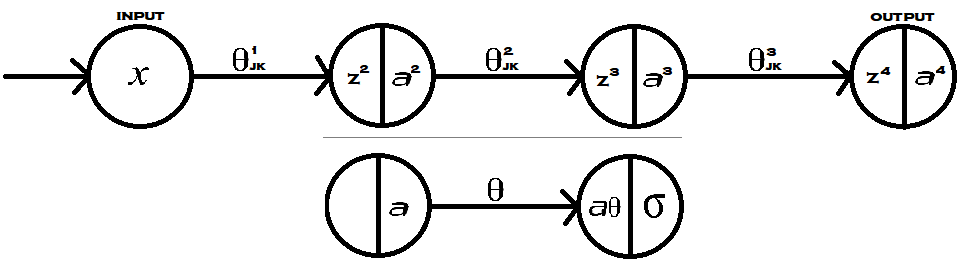
\includegraphics[scale=0.548]{onedimension}
\textbf{Figure 3.} A simple one input, two feature neural network, without a bias. \\ \\
The figure includes a simple one input, one feature neural network, without a bias, to give further intutition. The network takes in an input, $x$, in the first layer. Then to determine the activation value of the second layer, the hypothesis function $h_{\boldsymbol{\Theta}} = x \times \theta_{jk}^1$ gets employed. The value is denoted $z^l_j$ for convenience, l being for layer and j being for identifying the neuron. In this case, the indication $jk$ does not matter as there is only one neuron per layer. However, $z^l_j$ then gets ran through the sigmoid function for the complete activation value, denoted $a^l_j$. The process continues, as between the second and third layer the figure showcases the process in further depth. The value $a^l_j$, from our previous neuron, gets multiplied by the weight inbetween them, $\theta_{jk}^2$, and then put through the activation function once again to determine the activation value for the neuron. The process continues until the output, where the model's prediction would be displayed. 
\\ The backpropagation in this case for our first weight, the one that affects everything in our system, would be the derivative \cite{backpropagation}:
\[\frac{\partial J(\boldsymbol{\Theta})}{\partial \theta_{jk}^1} \ \text{where} \ J(\boldsymbol{\Theta}) = J(\theta_0, \theta_1, \theta_2,...,\theta_n)\] 
The cost function $J(\boldsymbol{\Theta})$ is a function of all of the weights to the system. However, in order to compute this derivative the chain rule has to be employed, as:
\[\frac{\partial J(\boldsymbol{\Theta})}{\partial \theta_{jk}^1} = \frac{\partial J(\boldsymbol{\Theta})}{\partial a^4} \times \frac{\partial a^4}{\partial z^4} \times \frac{\partial z^4}{\partial a^3} \times \frac{\partial a^3}{\partial z^3} \times \frac{\partial z^3}{\partial a^2} \times \frac{\partial a^2}{\partial z^2} \times \frac{\partial z^2}{\partial \theta^1_{jk}}\]
\[\frac{\partial J(\boldsymbol{\Theta})}{\partial \theta_{jk}^1} = \frac{\partial \frac{1}{2}(a^4 - y)^2}{\partial a^4} \times \frac{\partial \sigma(z^4)}{\partial z^4} \times \frac{\partial (a^3\theta^3_{jk})}{\partial a^3} \times \frac{\partial \sigma(z^3)}{\partial z^3} \times \frac{\partial (a^2\theta_{jk}^2)}{\partial a^2} \times \frac{\partial \sigma(z^2)}{\partial z^2} \times \frac{\partial (x\theta_{jk}^1)}{\partial \theta_{jk}^1}\]
\[\frac{\partial J(\boldsymbol{\Theta})}{\partial \theta_{jk}^1} = (a^4 - y) \times \sigma'(z^4) \times \theta_{jk}^3 \times \sigma'(z^3) \times \theta_{jk}^2 \times \sigma'(z^2) \times x\]
The same method would have to be applied to all of the weights and biases in our system. In order to minimize the weight $\theta_{jk}^1$ in the system, the derivative would be plugged into the gradient descent algorithm for the specific training example as follows:
 \[\theta_{jk}^1 = \theta_{jk}^1 - \alpha \frac{\partial}{\partial\theta_{jk}^1} J(\boldsymbol{\Theta})\]
\[\theta_{jk}^1 = \theta_{jk}^1 - \alpha ((a^4 - y) \times \sigma'(z^4) * \theta_{jk}^3 \times \sigma'(z^3) \times \theta_{jk}^2 \times \sigma'(z^2) \times x)\]
\[\theta_{jk}^1 = \theta_{jk}^1 - \alpha ((a^4 - y) \times \sigma(z^4)(1-\sigma(z^4)) \times \theta_{jk}^3 \times \sigma(z^3)(1-\sigma(z^3)) \times \theta_{jk}^2 \times \sigma(z^2)(1-\sigma(z^2)) \times x)\]
\\
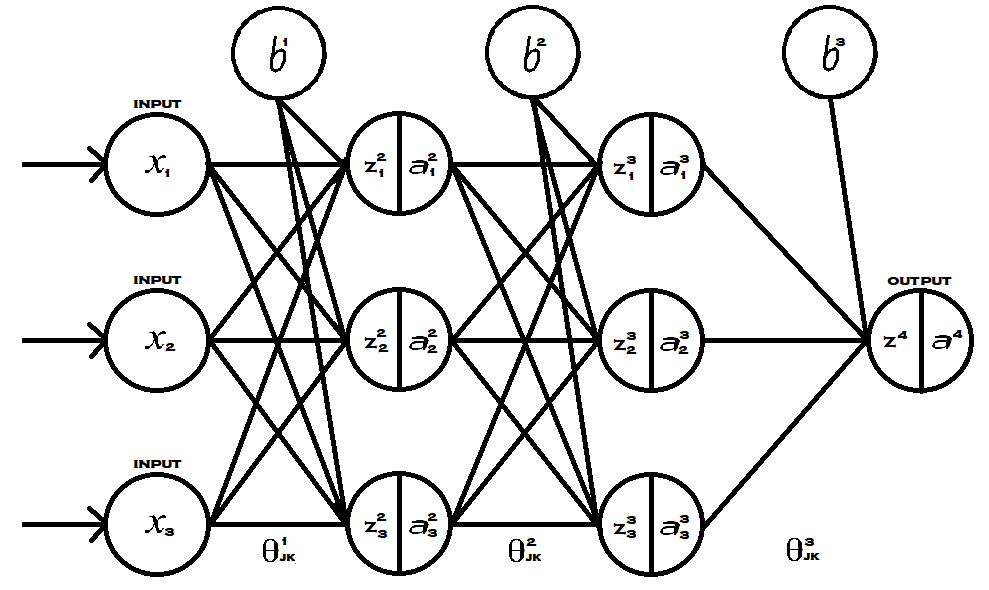
\includegraphics[scale=0.548]{multidimension}
\textbf{Figure 3.} A more complex neural network, now including biases and multiple neurons per layer.. \\ \\
Increasing the layers in the network, the same principles can be used. To find the derivative of the error function with respect to a weight in the first layer, the chain rule is employed. There are further steps that need to be ensured, however. Backtracking to the weight $\theta^1_{22}$, or the weight connecting the input $x_2$ to the neuron $z^2_2$, would be denoted as the derivative:
\[\frac{\partial J(\boldsymbol{\Theta})}{\partial \theta^1_{22}}\]
Backpropagating through to layer 4 is nothing different than from before, and means:
\[\frac{\partial J(\boldsymbol{\Theta})}{\partial \theta^1_{22}} = \frac{\partial J(\boldsymbol{\Theta})}{\partial a^4} \times \frac{\partial a^4}{z^4} \times \frac{z^4}{\partial \theta_{22}^1}\]
\[\frac{\partial J(\boldsymbol{\Theta})}{\partial \theta^1_{22}} = (a^4 - y) \times \sigma'(z^4) \times \frac{z^4}{\partial \theta_{22}^1}\]
To expand on the last derivative, in layer 3 the process changes, as all three of the connections made need to taken into account:
\[\frac{z^4}{\partial \theta_{22}^1} = \sum_{j=1}^3 \frac{\partial z^4}{a^3_j} \times \frac{\partial a^3_j}{\partial z^3_j} \times \frac{\partial z^3_j}{\partial \theta_{22}^1}\]
Individually, these make:
\[\frac{\partial z^4}{a^3_j} = \frac{\partial}{\partial a^3_j} b^3 + a^3_j\theta^3_{j1} = \theta^3_{j1}\]
\[\frac{\partial a^3_j}{\partial z^3_j} = \frac{\partial }{\partial z^3_j} \sigma(z^3_j) = \sigma'(z^3_j) = \sigma(z^3_j)(1-\sigma(z^3_j))\]
That makes our initial derivative:
\[\frac{\partial J(\boldsymbol{\Theta})}{\partial \theta^1_{22}} = (a^4 - y) \times \sigma'(z^4) \times \sum_{j=1}^3 \Big[\theta^3_{j1} \times \sigma'(z^3_j) \times \frac{\partial z^3_j}{\partial \theta^1_{22}}\Big]\]
Then moving into layer 2, using the similar approach. However, given that layer 2 has three possible connections for the weight, the sum of them is introduced:
\[\frac{\partial z^3_j}{\partial \theta^1_{22}} = \sum_{j=1}^{3} \frac{\partial z^3_j}{a^2_2} \times \frac{a^2_2}{z^2_2} \times \frac{z^2_2}{\theta_{22}^1}\]
\[\frac{\partial z^3_j}{\partial \theta^1_{22}} = \sum_{j=1}^{3} \theta^2_{j2} \times \sigma'(z^2_j) \times \frac{z^2_2}{\theta_{22}^1}\]
The initial derivative is now set at:
\[\frac{\partial J(\boldsymbol{\Theta})}{\partial \theta^1_{22}} = (a^4 - y) \times \sigma'(z^4) \times \sum_{j=1}^3 \Big[\theta^3_{j1} \times \sigma'(z^3_j) \times \sum_{j=1}^{3} \Big[ \theta^2_{j2} \times \sigma'(z^2_2) \times \frac{\partial z^2_2}{\partial \theta_{22}^1}\Big]\Big]\]
The last layer is now left, to find the derivative of the cost function with respect to the weight $\theta_{22}^1$:
\[\frac{z^2_2}{\theta_{22}^1} = \frac{\partial}{\partial \theta_{22}^1} \ b^1 + x_1\theta_{21}^1 + x_2\theta_{22}^1 + x_3\theta^1_{23} = x_2\]
The complete computation for the weight $\theta_{22}^1$ is therefore: 
\[\frac{\partial J(\boldsymbol{\Theta})}{\partial \theta^1_{22}} = (a^4 - y) \times \sigma'(z^4) \times \sum_{j=1}^3 \Big[\theta^3_{j1} \times \sigma'(z^3_j) \times \sum_{j=1}^{3} \Big[ \theta^2_{j2} \times \sigma'(z^2_2) \times x_2\Big]\Big]\]
A more general form for any weight in the first layer could also be devised, such that layer 2 takes on further general values, given a neuron $k$:
\[\frac{\partial J(\boldsymbol{\Theta})}{\partial \theta^1_{jk}} = (a^4 - y) \times \sigma'(z^4) \times \sum_{j=1}^3 \Big[\theta^3_{j1} \times \sigma'(z^3_j) \times \sum_{j=1}^{3} \Big[ \theta^2_{jk} \times \sigma'(z^2_j) \times \sum_{j=1}^3x_j\Big]\Big]\]
As such, the gradient descent algorithm for $\theta_{jk}^1$ would then be:
\[\theta_{jk}^1 = \theta_{jk}^1 - \alpha\Big((a^4 - y) \times \sigma'(z^4) \times \sum_{j=1}^3 \Big[\theta^3_{j1} \times \sigma'(z^3_j) \times \sum_{j=1}^{3} \Big[ \theta^2_{jk} \times \sigma'(z^2_j) \times \sum_{j=1}^3x_j\Big]\Big]\Big)\]
The same can be done for the bias, $b^1$ in layer 1. However, instead of deriving with respect to the weight, the cost function is derived with respect to the bias:
\[\frac{\partial J(\boldsymbol{\Theta})}{\partial b^1} = (a^4 - y) \times \sigma'(z^4) \times \sum_{j=1}^3 \Big[\theta^3_{j1} \times \sigma'(z^3_j) \times \sum_{j=1}^{3} \Big[ \theta^2_{jk} \times \sigma'(z^2_j) \times \frac{\partial z^2_j}{\partial b^1}\Big]\Big]\]
\[\frac{\partial z^2_j}{\partial b^1} = \frac{\partial}{\partial b^1} \ b^1 + x_1\theta_{21}^1 + x_2\theta_{22}^1 + x_3\theta^1_{23} = 1\]
\[\frac{\partial J(\boldsymbol{\Theta})}{\partial b^1} = (a^4 - y) \times \sigma'(z^4) \times \sum_{j=1}^3 \Big[\theta^3_{j1} \times \sigma'(z^3_j) \times \sum_{j=1}^{3} \Big[ \theta^2_{jk} \times \sigma'(z^2_j)\Big]\Big]\]

\section{Conclusion}
The process of minimizing the error function is a large process, and gets larger depending on the amount of features the network includes. However, there are some similarities that stay true when it comes to finding the optimal weights, such as the correlation between finding the derivative using backpropagation and the gradient descent algorithm, along with the similarities within the equations themselves. The intuition behind these processes is surprisingly simple, given the level of mathematics, but that is what makes it so captivating.

\begin{thebibliography}{9}
\bibitem{patternml}
Bishop, C.M. (2006). \textit{Pattern Recognition and Machine Learning}. Retrieved from http://users.isr.ist.utl.pt/~wurmd/Livros/school/Bishop\%20-\%20Pattern\%20Recognition\%20And\%20Machine\%20Learning\%20-\%20Springer\%20\%202006.pdf

\bibitem{convex}
Breckbaldwin. (2009). Convexity of (Root) Mean Square Error, or Why Committees Won the Netflix Prize. Retrieved from https://lingpipe-blog.com/2009/09/29/convexity-of-root-mean-square-error-or-why-committees-won-the-netflix-prize/

\bibitem{nndef} 
BusinessDictionary. (n.d.). What is neural network? definition and meaning. Retrieved from http://www.businessdictionary.com/definition/neural-network.html

\bibitem{sumrule}
Dawkins, P. (n.d.). Calculus I - Proof Of Various Derivative Properties. Retrieved from http://tutorial.math.lamar.edu/Classes/CalcI/DerivativeProofs.aspx

\bibitem{backpropagation}
Kapur, R. (2016). Rohan \& Lenny \#1: Neural Networks \& The Backpropagation Algorithm, Explained. Retrieved from https://ayearofai.com/rohan-lenny-1-neural-networks-the-backpropagation-algorithm-explained-abf4609d4f9d

\bibitem{normal}
Kapur, R. (2016). Rohan \#3: Deriving the Normal Equation using matrix calculus. Retrieved from https://ayearofai.com/rohan-3-deriving-the-normal-equation-using-matrix-calculus-1a1b16f65dda

\bibitem{deeplearning}
Nielson, M.A. (2015). \textit{Neural Networks and Deep Learning}. Retrieved from http://neuralnetworksanddeeplearning.com



\end{thebibliography}
\end{document}
